\section*{Имитационные эксперименты}
\addcontentsline{toc}{section}{Имитационные эксперименты}
\subsection*{Варьирование параметров -- SD-модель}
\addcontentsline{toc}{subsection}{Варьирование параметров -- SD-модель}

\textbf{Задание:}\\
Создать интерфейс модели SIR, позволяющий изменять количество агентов, параметры модели до запуска эксперимента. Создать эксперимент варьирования параметров. Визуализировать динамику инфицированных в зависимости от значения параметров.\\

\textbf{Решение:}\\
Изначально необходимо создать эксперимент варьирования параметров в окне проекта.\\

В качестве параметра варьирования был выбран параметр \textit{beta}. (Рисунок \ref{fig:var_sir1})
\begin{figure}[h]
	\centering 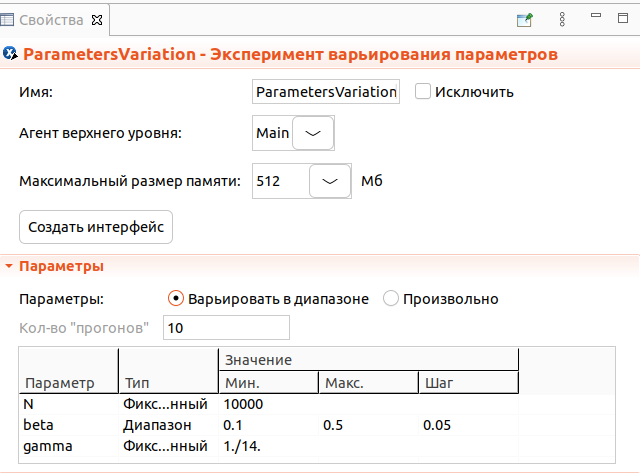
\includegraphics[scale=0.3]{var_sir1}
	\caption{Варьируемые параметры модели}
	\label{fig:var_sir1}
\end{figure}

Также необходимо создать интерфейс эксперимента. (Рисунок \ref{fig:var_sir2})
\begin{figure}[h]
	\centering 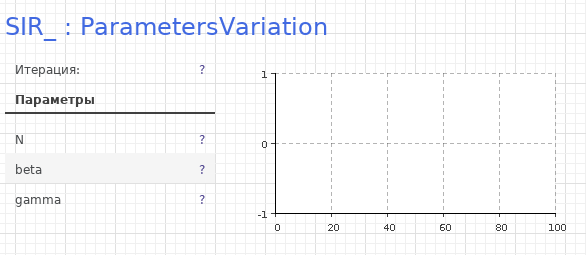
\includegraphics[scale=0.5]{var_sir2}
	\caption{Интерфейс варьирования эксперимента}
	\label{fig:var_sir2}
\end{figure}

\newpage

Для добавления графика в интерфейс  создадим набор данных для накопителя инфицированных людей. При запуске эксперимента будут получены графики, характеризующие изменение объема накопителя в зависимости от параметра \textit{beta}. (Рисунок \ref{fig:var_sir3})
\begin{figure}[h]
	\centering 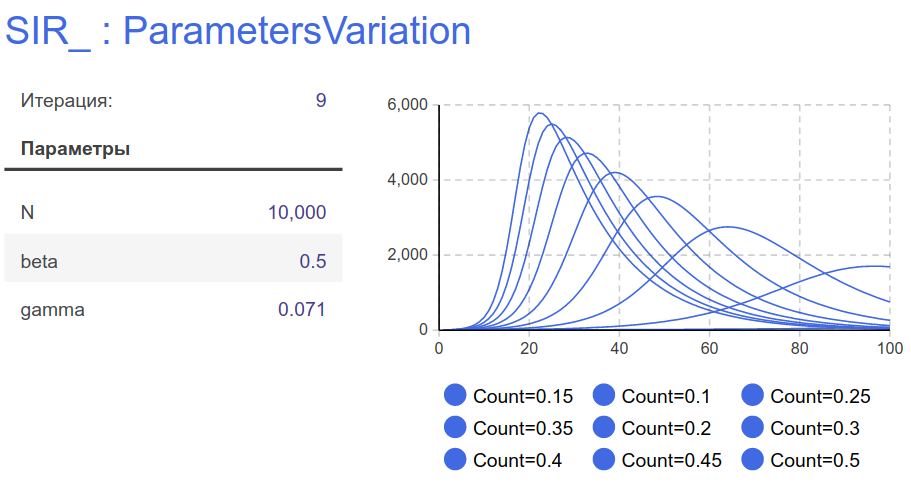
\includegraphics[scale=0.5]{var_sir3}
	\caption{Изменение объёма накопителя инфицированных людей}
	\label{fig:var_sir3}
\end{figure}

Таким образом, был создан эксперимент варьирования параметров для системной модели, на примере которой были рассмотрены основные механики экспериментов варьирования параметров и их интерфейсов. 